Following the design phase, it is crucial to test the protocol in a practical environment in order to verify that it works as intended. Furthermore,
extensive performance evaluations need to be conducted to assure the viability of the devised techniques. Both of these tasks are achieved through
thorough software simulation. For this purpose, a dedicated, cycle-accurate simulator was implemented that supports the designed protocol with all the
features described in Chapter \ref{ch:protocol}.

The simulator is written in C++ and based on the \textit{\omnet{}} discrete event simulation framework \cite{omnet}. \omnet{} provides a general-purpose
network simulation architecture and promotes a modular design. In general, it allows the programmer to define the components of the network via a
special scripting language called \textit{NED}. With NED files, modules may be specified as they appear from the outside, by means of parameters,
gates, and connections. Furthermore, a module is allowed to have any number of submodules, facilitating a hierarchical structure. A C++
class is assigned to each module that controls the component's internal behavior together with the parameters. The gates define the ports of the
module through which it sends and receives messages. The connections link the gates of different modules (or submodules) together and thus define the
message flows and the network's topology.

The simulator makes extensive use of the hierarchical and modular approach of \omnet{}. The processing elements, network interfaces, and routers are
defined as modules and instanced as many times as required, depending on the \gls{noc} dimensions. They are interconnected through their gates and
arranged in a way mirroring the structure of the \gls{noc}. To create a simulation as realistic as possible, they are made up of a number of
submodules, such as queues, buffers, and crypto modules, resembling the actual hardware layout.

%\omnet allows the user to record detailed statistics. Used as basis for the evaluation in Chapter \ref{ch:evaluation}.

In Section \ref{sec:generalass}, fundamental assumptions about the simulation environment are presented. Subsequently, Section
\ref{sec:componentstructure} elaborates on the hierarchical structure of the components and their layout. Finally, an overview of the various
configurable parameters of the simulator is given in Section \ref{sec:confparams}.

\section{General Assumptions}\label{sec:generalass}
\subsection{The GALS Paradigm}
In Section \ref{sec:networkonchipfun}, it was mentioned that \glspl{noc} lend themselves well to the implementation of the \gls{gals} design paradigm.
For the simulation, it was not considered for three reasons. First, its usage requires the existance of multiple clock domains: each core runs with the
frequency best suited for itself and is not synchronized with other cores in the network (\enquote{globally asynchronous}). This, however, is very
finical to implement correctly. Second, since the cores themselves each operate under a single clock (\enquote{locally synchronous}), \gls{gals} would
only affect the transmissions from one router to another. Third, the cores are assumed to be identical and hence run with the same frequency anyway.
On these grounds, a globally synchronous architecture with a single clock driving all components is used in the simulator.

\subsection{Clock Frequency}
The \gls{noc}'s global clock runs at a frequency of 500 MHz as this is a common speed in \gls{noc}-related research
\cites{frey15stateobfuscation}{frey17hardenednoc}. Unfortunately, the PRINCE cipher that is employed for all cryptographic operations is unable to run at
such a high frequency. However, in Section \ref{subsubsec:prince} it was shown that the algorithm runs flawlessly at frequencies of up to 250 MHz.
Thus, the crypto modules operate at half the frequency of the \gls{noc}, with every two cycles of the global clock corresponding to one
cycle for the crypto modules. Hence, the processing of a single block with PRINCE is assumed to take two clock cycles in the simulator.

It was mentioned above that the integration of multiple clock domains is very finical. However, when they are not independent and the global clock's
frequency is evenly divisible by the required frequency, as is the case for the crypto modules, this becomes significantly easier. Here, a new clock
is derived from the global clock that simply omits every other tick.

\subsection{Single Cycle Routing}
The number of cycles required for routing\footnote{Routing refers to the whole process from receiving a flit on an input port to forwarding it on the
appropriate output port, including route calculation, switch allocation, and switch traversal \cite[see][2]{routinglectureutah}.} is a key factor to the
overall performance of the \gls{noc}. While four cycle \cite[e.g.][]{routinglectureutah} and two cycle routing \cite[e.g.][]{lu11nocrouter} are
popular approaches, architectures requiring only a single cycle have also proven to be both feasible and practical
\cites{hayenga09scarab}{ved17routeonfly}.

As achieving low latencies is of utmost importance for this thesis, single cycle routing is implemented in the simulator. Such an approach is easily
able to operate at the required frequency of 500 MHz \cite[7]{hayenga09scarab}. Furthermore, high routing speeds imply less required buffers
\cite[1]{ved17routeonfly}, reducing the occupied chip area of the routers. Although completely bufferless architectures are possible
\cite{hayenga09scarab}, the implemented scheme grants each router one input buffer per port (i.e., five buffers per router) in order to prevent
immediate discarding of flits in the case of link congestions. Output buffers, however, are not used.

In order for the complexity of the simulator to stay within manageable bounds, the internal structure of the routers is kept simple. For instance, no
virtual channels are used for the input buffers mentioned above. This, however, implies that a flit delayed by a congestion of the targeted output
link also holds back all following flits in the buffer, even if they would be routed to a different link.

\section{Component Structure}\label{sec:componentstructure}
This section provides an in-depth view on the modular structure of the simulator. In a top-down approach, it begins with the outermost layer of the
hierarchy (i.e., the \gls{noc} itself) and then descends into the individual components. The figures used to support the textual explanations are
drawn directly from the graphical interface provided by \omnet{}.

\subsection{Complete Network}
The structure of the \gls{noc} in the simulator mirrors the 2D mesh topology of the network (cf. Figure \ref{fig:nocexample}). The only difference
here is that the network interfaces are not built as submodules of the processing elements, but as independent components interposed between the
processing elements and routers. Figure \vref{fig:omnetnoc} visualizes this approach.

\begin{figure}
    \centering
    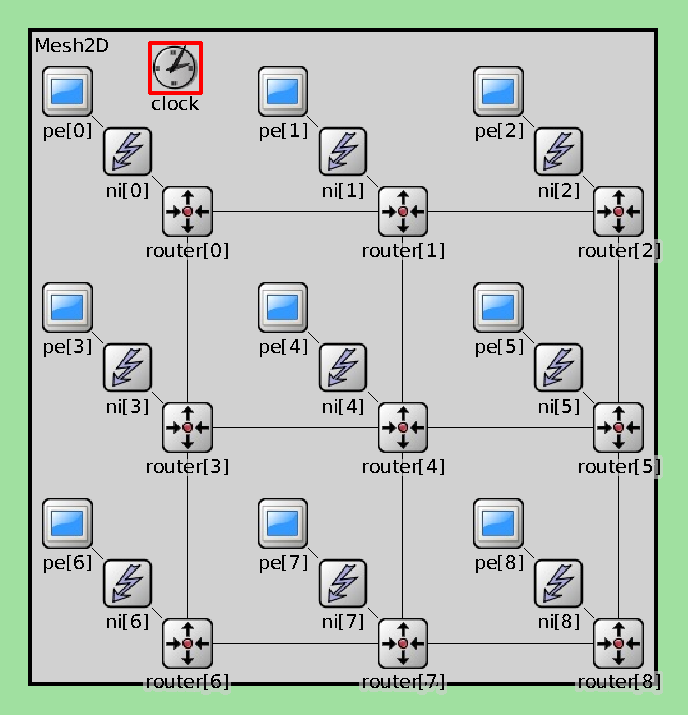
\includegraphics[width=0.5\textwidth]{omnet-noc}
    \caption[Simulator view of the NoC]{The \gls{noc} as it appears in \omnet{}. For clarity reasons, it was truncated to a 3x3 mesh. Each processing
    element, network interface, and router are assigned an index for simulation purposes. The network interfaces were not integrated into the
    processing elements to allow for better visualizations of the traffic flow.}
    \label{fig:omnetnoc}
\end{figure}

In addition to these familiar components, the global clock is also implemented as its own module. As a part of the simulation, it drives all other
modules and their submodules through signals. Any module may attach itself to this clock by registering as a receiver for the appropriate signal.

\subsection{Processing Element}
The processing element is a very plain component from the perspective of the simulator. It contains nothing more than a traffic generator and a flit
consumer with an input queue. Figure \vref{fig:omnetpe} depicts its appearance in \omnet{}.

\begin{figure}
    \centering
    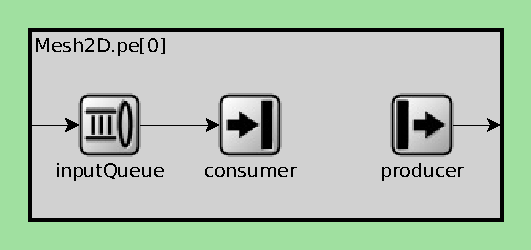
\includegraphics[width=0.5\textwidth]{omnet-pe}
    \caption[Simulator view of the processing element]{An instance of a processing element module of \omnet{}. A traffic generator (producer) randomly
    creates flits and sends them to the connected network interface. Flits arriving from the network interface are accepted by a pseudo-buffer
    (inputQueue) that subsequently passes them to the consumer.}
    \label{fig:omnetpe}
\end{figure}

The traffic generator randomly produces flits and sends them to the network interface. On each clock tick, one flit is created with a configurable
\textit{generation probability}. The destination is chosen at random from the set of network nodes (excluding the own node) with a uniform
distribution. The produced flits are always data flits (not \glspl{mac} or \glspl{arq}) without any meaningful information contained in their
payloads\footnote{For the simulation, only the transmission parameters are of interest, not the actual data being transferred.}. Furthermore, the
generator may be configured to always produce a pair of two flits: in the event of a flit creation as described above, another flit will always be
produced on the next clock tick with the same destination. The purpose of this generation pattern is to allow for a fair comparison of uncoded and
network coded protocol variants and explained in detail in Section (insert ref here).

The flit consumer simply accepts any flits arriving from the local network interface and records these events with \omnet{}'s statistics system. Since
the flits are of no further use after this, they are subsequently destroyed. An input buffer is located in front of the consumer to ensure both
synchronization with the global clock and that the travel time from network interface to processing element is precisely one cycle.

\subsection{Network Interface}
The network interface is the most complex part of the simulator. Implementing all the logic required by the protocol, it contains several crypto
modules, network coding components, the retransmission buffer as well as the verification and \gls{arq} infrastructure. The layout of these components
slightly differs for each variant. However, all variants resemble the structure of their corresponding flowchart in Section \ref{sec:theprotocol}, so
explaining the network interface by means of one variant is deemed sufficient. For this purpose, the network coded interwoven authentication version
is described below. Figure \vref{fig:omnetni} shows the internal structure as rendered by \omnet{}'s graphical interface.
% 1 paragraph per component
% at the end: table with all components, their delay (cycles)

\begin{figure}
    \centering
    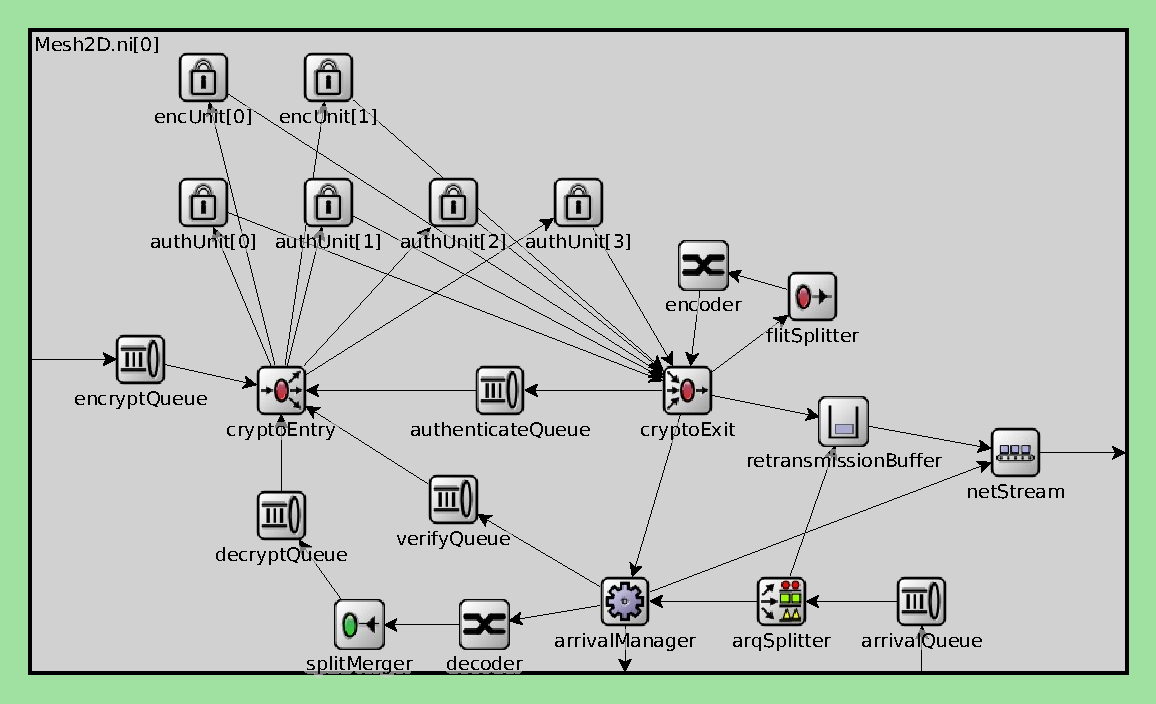
\includegraphics[width=0.9\textwidth]{omnet-ni}
    \caption[short]{long}
    \label{fig:omnetni}
\end{figure}

The network interface was modeled as accurately as possible to be able to evaluate internal congestions like competition of multiple flits over the
available crypto modules.

Figure X shows the internal structure of the network interface as rendered by \omnet{}'s graphical interface.

\subsubsection{Crypto Modules}
- Access Priorities (1. sender in order to not tear apart a generation and provoke timeouts at the receiver, 2. receiver)

Encryption/Decryption:
1 input block = 2 cycles for all methods

Authentication:
Ind. Auth 3 input blocks → 6 cycles
Int. Auth 2 input blocks → 4 cycles + 1 cycle for authcode generation → 5 cycles (2x as many authcodes generated as for ind. auth)
Gen. Auth 5 input blocks → 10 cycles (half as many MACs generated as for ind. auth)

\subsubsection{Retransmission Buffer}
% No auth. for ARQs: RT doesn't know if an ARQ was modified and may send out false retransmission. To simplify, modified ARQs are ignored by the RT.

\begin{table}
    \centering
    \begin{tabulary}{\textwidth}{R|L}
        Component & Delay in cycles \\\hline
        Encryption/decryption & 2 \\
        Encoding (G2C3) & 3 (1 per combination) \\
        Encoding (G2C4) & 4 (1 per combination) \\
        Authentication (individual) & 6 \\
        Authentication (interwoven) & 5 \\
        Authentication (full gen.) & 10 \\
        Storing flit in \gls{rtb} & 1 \\
        Decoding & 2 (1 per flit) \\
        Comparing \glspl{mac} & 1 \\
        Composing an \gls{arq} & 1 \\
        \Gls{rtb} lookup & 2 (uncoded), 3 (coded)
    \end{tabulary}
    \caption[short]{long}
    \label{tab:processinglatencies}
\end{table}

\subsection{Routers}
% Only input buffers → single cycle routing
% Routing is only performed when receiving router's input queue is not full

\begin{table}
    \centering
    \begin{tabulary}{\textwidth}{R|L}
        Transmission & Delay in cycles \\\hline
        PE ←→ NI & 1 \\
        NI ←→ Router & 1 \\
        Router ←→ Router & 1
    \end{tabulary}
    \caption[short]{long}
    \label{tab:transmissionlatencies}
\end{table}

\section{Configurable Parameters}\label{sec:confparams}
- generation probability

\iffalse
\begin{itemize}
    \item Retransmission Buffer structure and lookup times
        \begin{itemize}
            \item corresponding flits are stored consecutively (e.g. data/MAC of same FID, flits of same generation etc.)
            \item lookup time (in clock cycles) is a parameter in the simulation
            \item UC case: one cycle lookup is fine (just need to find FID, mode field determines offset in the buffer)
            \item NC case: two cycles for lookup (one to find GID, one to compare GEVs of the generation in parallel, mode determines offset)
        \end{itemize}
    \item Priorities
        \begin{itemize}
            \item retransmission buffer: ARQs have priority
            \item crypto units (→ entry guard): arriving flits have priority
        \end{itemize}
    \item Buffers/Queues
        \begin{itemize}
            \item App/NI/Routers have only input buffers, no output buffers
            \item Routers only route flits when the receiving router's input queue is not full
        \end{itemize}
    \item Crypto units
        \begin{itemize}
            \item Separate units for encryption and authentication
            \item Encryption units can also decrypt → very easy to see with PRINCE
            \item Send/receive pipeline share the same set of crypto units
            \item Talk about auth. method 3: 32 bit block size, what algorithms?
            \item Latency: assume PRINCE → ~35MHz FPGA, *~4 for ASIC → paper. Look at PRINCE paper and survey paper for numbers
        \end{itemize}
    \item Tracking finished IDs: prevent repeat attacks, prevent re-processing a unit due to redundant retransmissions or repeat attacks, but still
        allow out-of-order arrivals SeemsGood
    \item Routing strategies: randomness needs hardware RNG → more complex logic, more area!

    \item Timeout of x (e.g. 8) cycles until first ARQ is sent
    \item The higher the ARQ timeout/limit, the less likely the flit is still in retransmission buffer
    \item → ARQ timeout/limit and retransmission buffer size have to correlate
\end{itemize}
\fi
